\begin{appendices}
\crefalias{chapter}{appendix}
%Some Table of Contents entry formatting
\addtocontents{toc}{\protect\renewcommand{\protect\cftchappresnum}{\appendixname\space}}
\addtocontents{toc}{\protect\renewcommand{\protect\cftchapnumwidth}{6em}}

%Begin individual appendices, separated as chapters
\chapter{Comparison of Acoustic Phonon Relaxation Rates in Silicon}
\label{app:si_relaxation_rates}
The accurate establishment of the bulk phonon relaxation times is an active research area involving experimental techniques and theoretical models ranging from first-principle to phenomenological approaches \cite{stokes_bulkSi_tau,RN273,RN217,ownNW,RN236}. Although initial theory assumed bulk relaxation times to be constant (i.e. frequency independent) the necessity for frequency-dependent times was realized and incorporated in the theoretical models. In recent years, first-principle approaches based on density-functional-theory (DFT) have provided theoretical predictions for the frequency-dependence of the bulk phonon relaxation times in a variety of materials including Silicon \cite{stokes_bulkSi_tau}. In this thesis, we use expressions obtained by assuming a $\omega^{-2}$ and  $\omega^{-4}$ dependence of relaxation times by Umklapp scattering and isotope scattering effects, respectively \cite{maldovan2011tf}. Optical modes are neglected, as owing to their low group velocities their contribution to thermal conductivity is low \cite{RN212}. 

The phonon relaxation times for bulk silicon at room temperature from various approaches are plotted in \Cref{fig:appendix-LA,fig:appendix-TA}. Overall, the different approaches yield the same range of relaxation times. The results show that models obtained by different approaches vary at very low frequencies, however it is important to note that low frequency phonons are non-dominant heat carriers in Si at room temperatures. The close agreement between the results from the approach used in this thesis (taken from Ref. \cite{maldovan2011tf}) and DFT calculations \cite{stokes_bulkSi_tau,RN244} especially for the transverse branch (dominant for heat transport) is noteworthy.

\begin{figure}[hbt]
	\centering 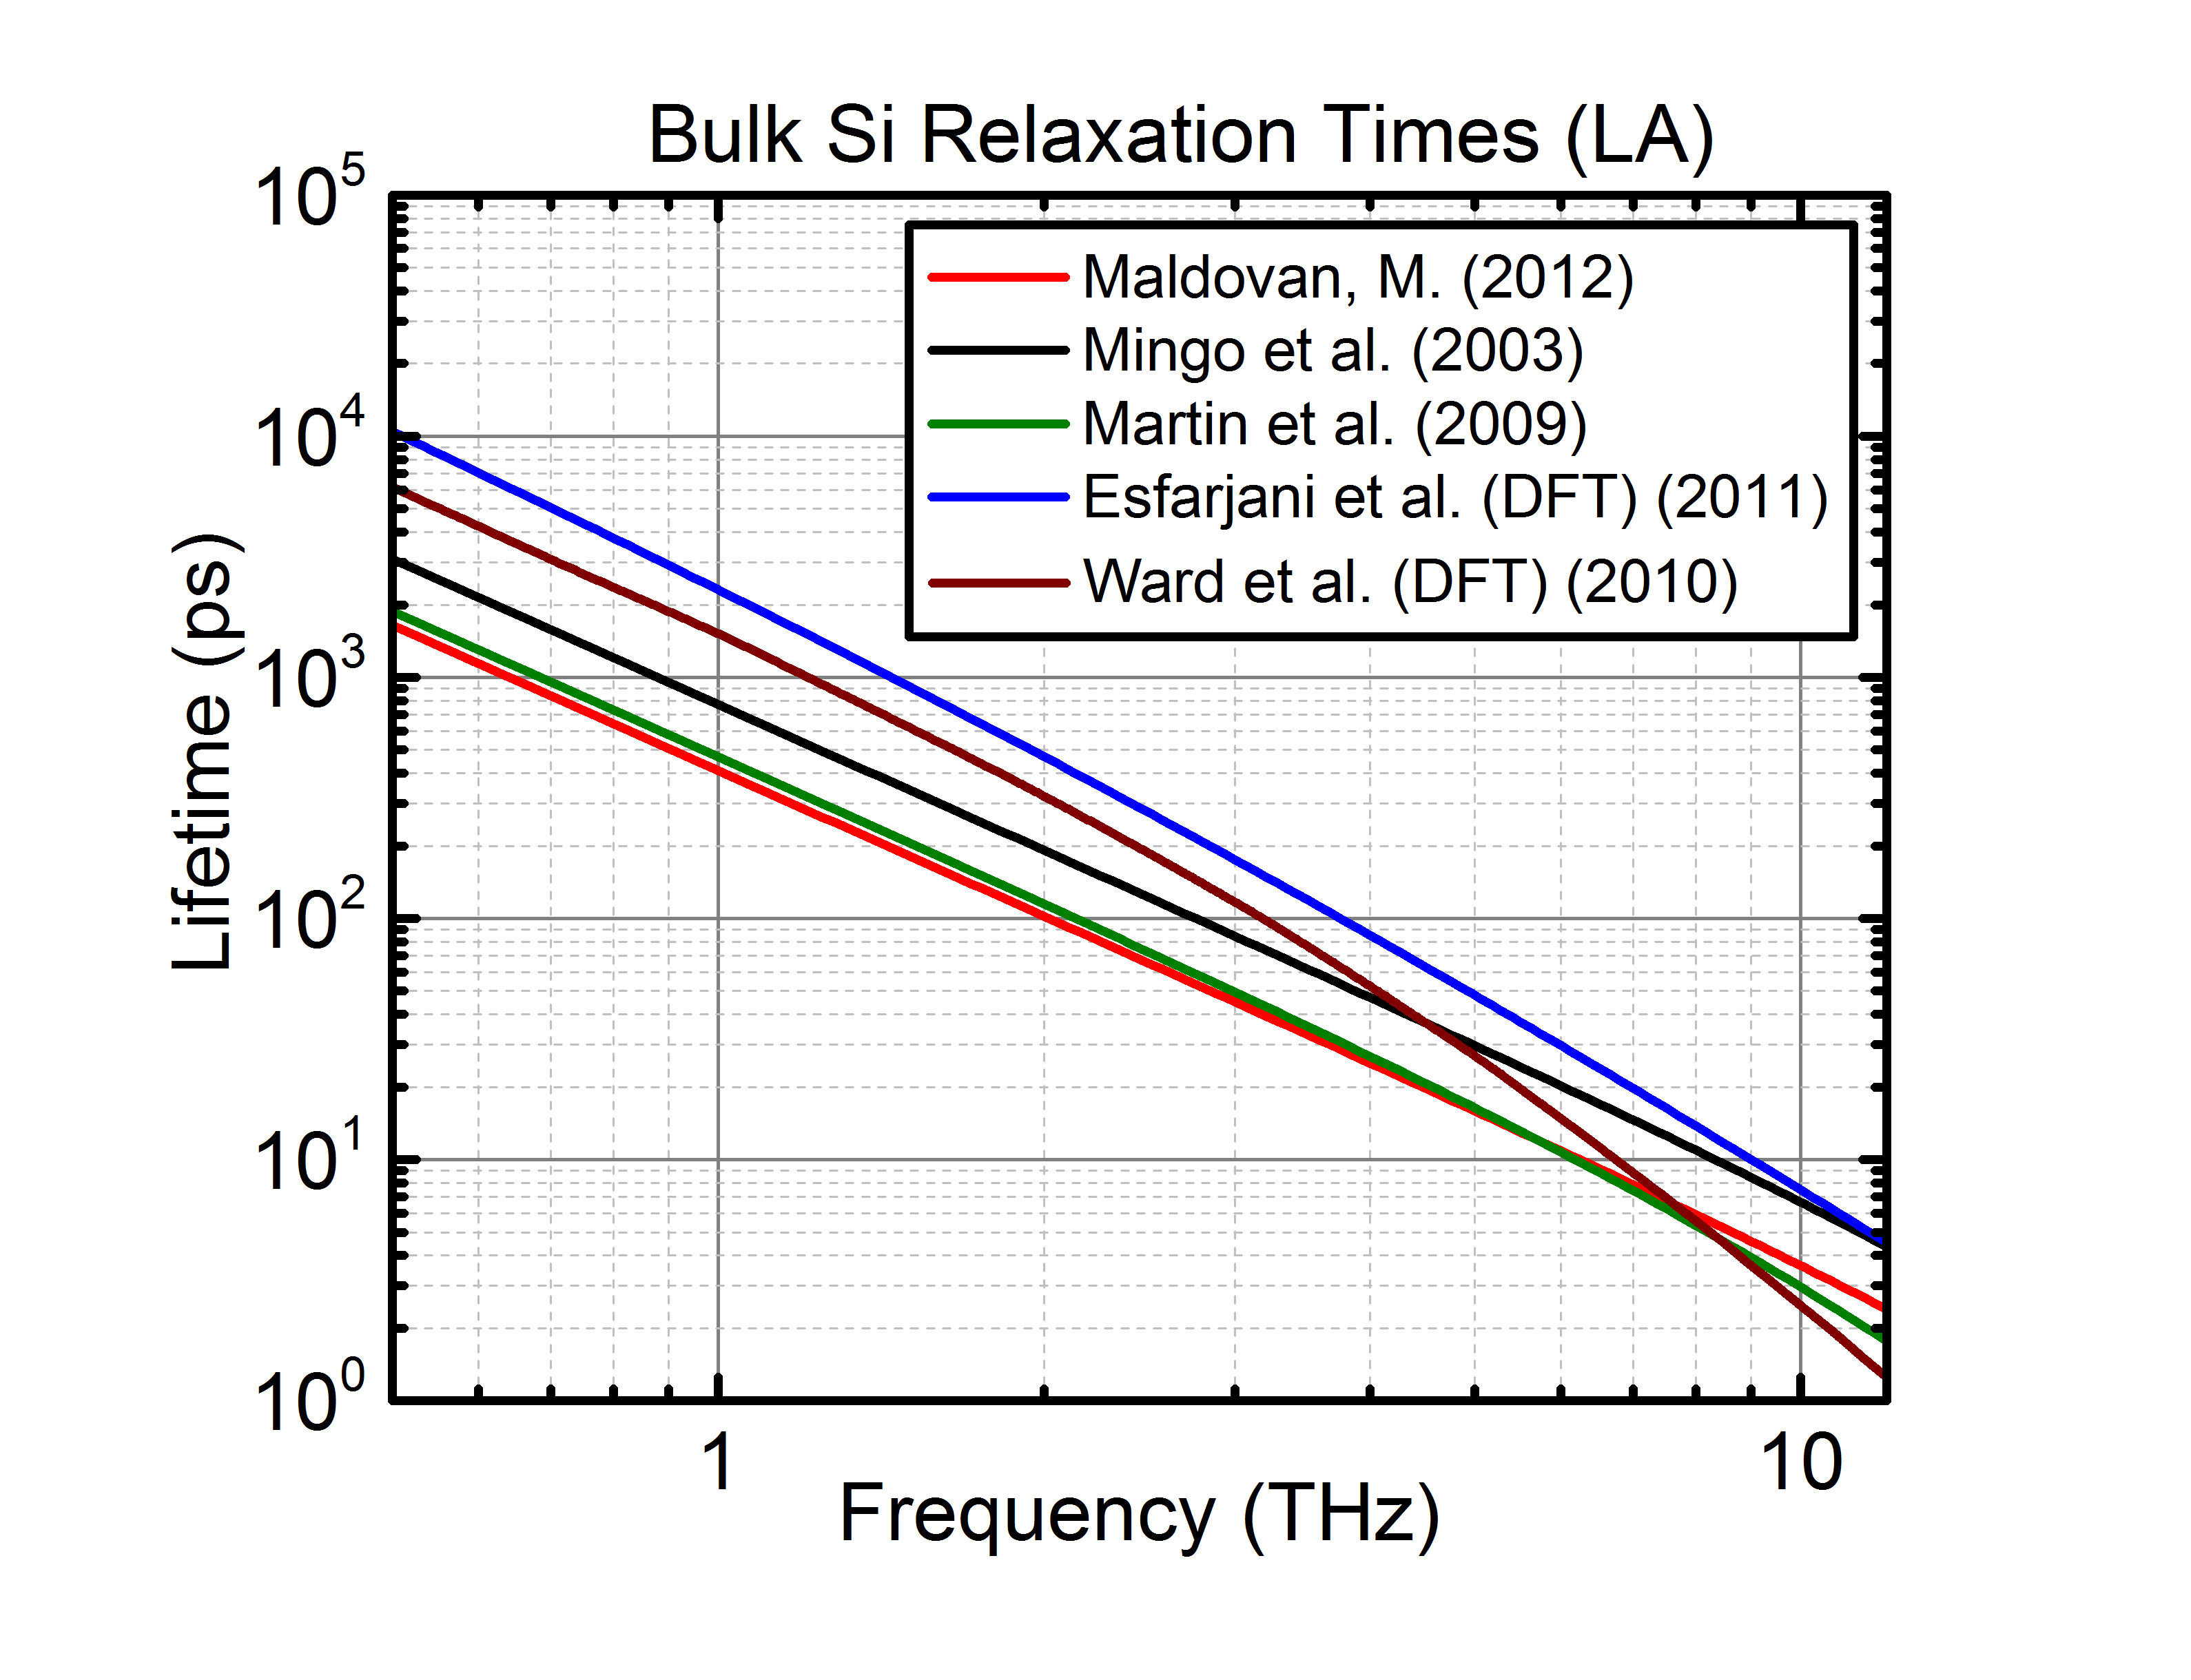
\includegraphics[width=0.80\textwidth]{/ch99/FigureA1.jpg}
	\caption{Relaxation times for longitudinal acoustic (LA) phonons in bulk Silicon at 300 K.}
	\label{fig:appendix-LA}
\end{figure}

\begin{figure}[hbt]
	\centering 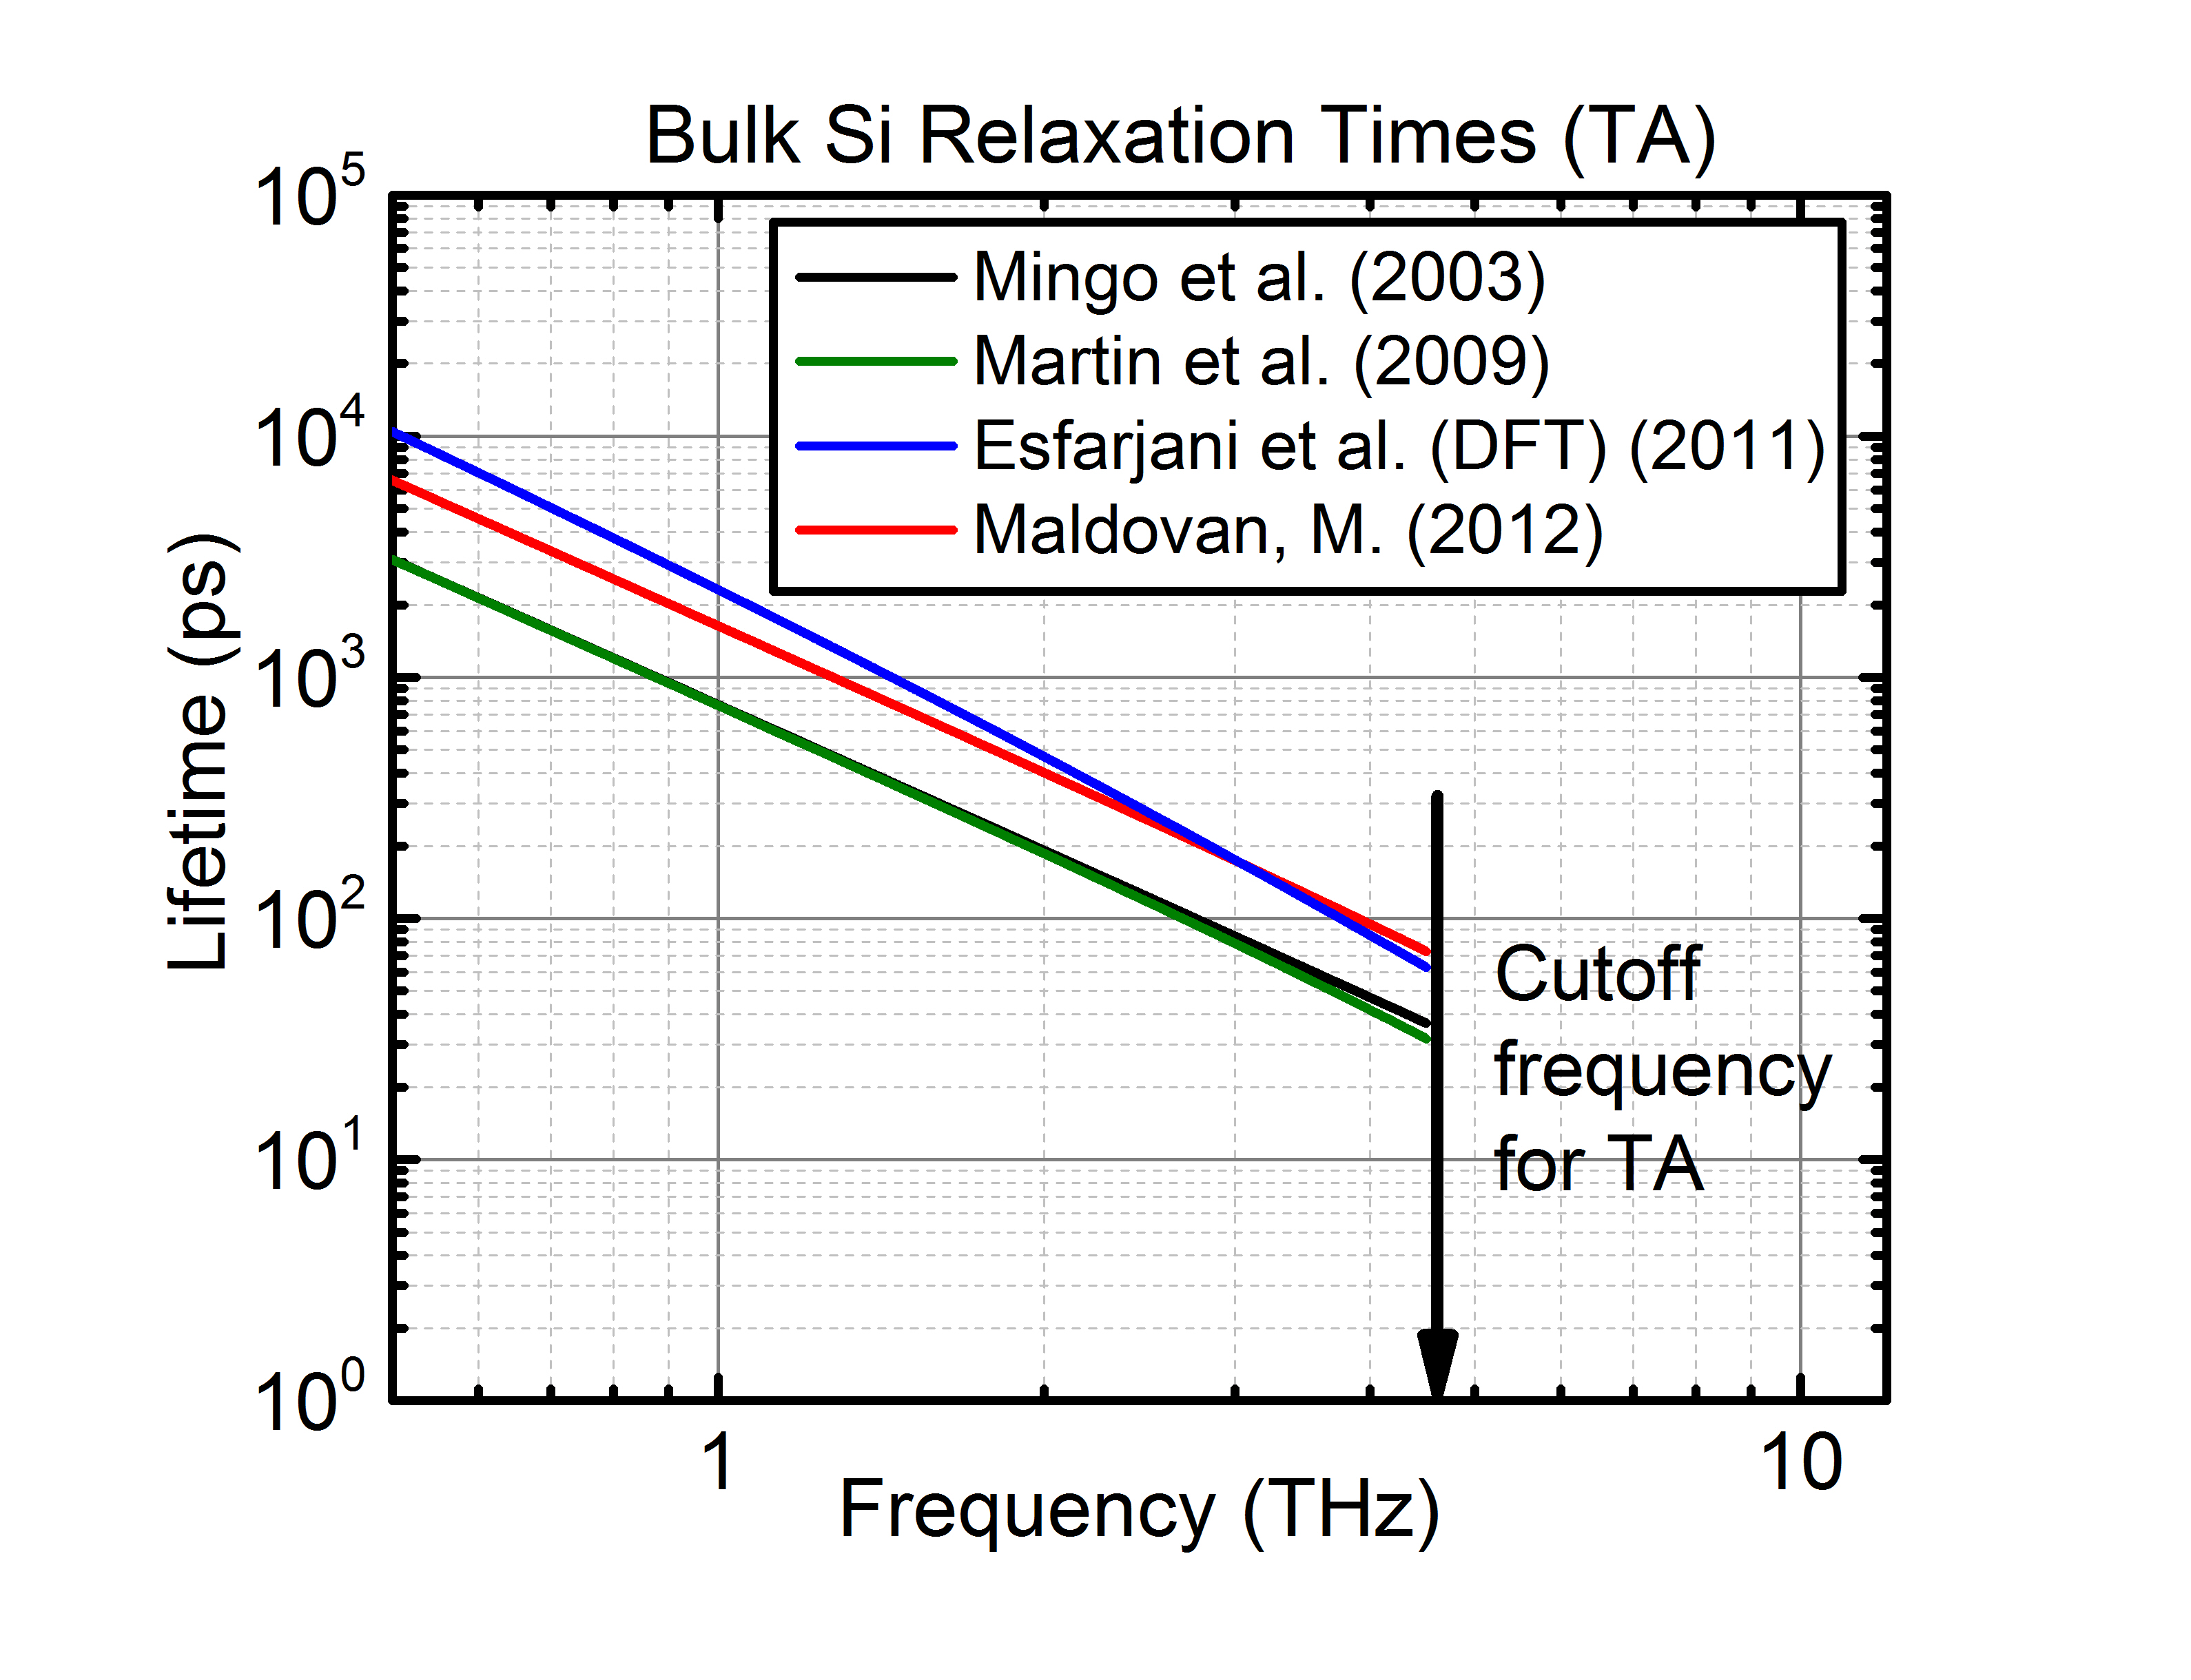
\includegraphics[width=0.80\textwidth]{/ch99/FigureA2.jpg}
	\caption{Relaxation times for transverse acoustic (TA) phonons in bulk Silicon at 300 K.}
	\label{fig:appendix-TA}
\end{figure}

%-------
\chapter{Numerical Calculations of Shadowing Function}
\label{app:shadowing}
A numerical calculation of shadowing function $S(\theta,\varphi)$ i.e. \Cref{eq:shadowing-full} is shown in \Cref{fig:appendix-Shadowing}. The plots are presented for two different cases: \gls{cl} = 5\gls{eta} (filled symbol) and \gls{cl} = 10\gls{eta} (open symbol). For smaller correlation lengths, the shadowing function approaches a lower value compared to a larger correlation length. This is intuitive and follows the previous discussion that a higher correlation length indicates a more continuous surface with lower number of sharp peaks and valleys, thus, reducing the number of points being shadowed. For incident angles close to the normal, a higher value of shadowing function is achieved, which is reasonable as the ability of a point to shadow a surface is negligible for small angles of incidence. It can also be seen in the case of higher correlation length, the value of shadowing quickly approaches unity for all incident angles less than \ang{70}. Note that the shadowing function used for calculations in our heat transport model is a subset of the general function presented. The locus generated by joining the points lying on the curves for which incident angles and observation angles are taken to be equal would provide the required shadowing function for the specular direction $S(\theta,\varphi=\theta)$.
\begin{figure}[hbt]
	\centering 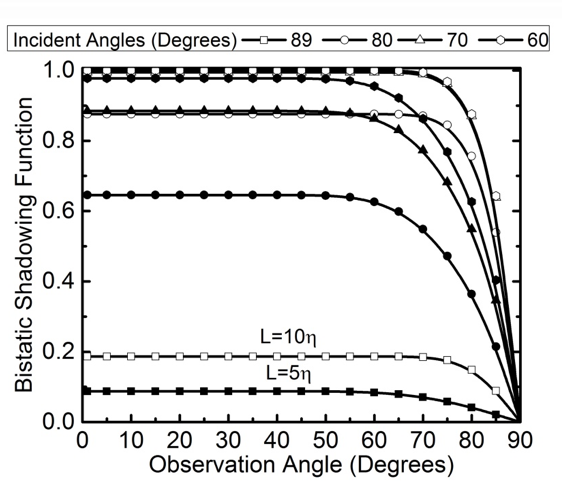
\includegraphics[width=0.85\textwidth]{/ch99/FigureB1.png}
	\caption{Bistatic shadowing function calculated for four representative incident angles and observation angles between 0 and $\pi$/2 radians. Open and filled symbols represent a surface correlation length \gls{cl} = 10\gls{eta} and \gls{cl} = 5\gls{eta}, respectively.}
	\label{fig:appendix-Shadowing}
\end{figure}
\end{appendices}